\subsection{Построение теней}

Как и упоминалось в аналитической части, карта теней представляет из себя совокупность матрицы преобразования координат в пространство координат источника света и матрицы глубин, вычисленной с точки зрения источника света. 

Вычисление матрицы глубин для карты теней использует упрощённую версию алгоритма с рисунка~\ref{fig:z-buffer}. Отличие заключается в том, что для карты теней не нужно заполнять матрицу цветов пикселей кадра. На вход поступают точки многоугольника, приведённые в пространство координат источника света. Вместо пространства координат экрана, используется пространство координат карты теней, которое использует ортогональную проекцию вместо перспективной.

Таким образом, алгоритм заполнения матрицы глубин для одного многоугольника изображён на рисунке~\ref{fig:smap_buffer}.

\begin{figure}[h!]
  \centering
  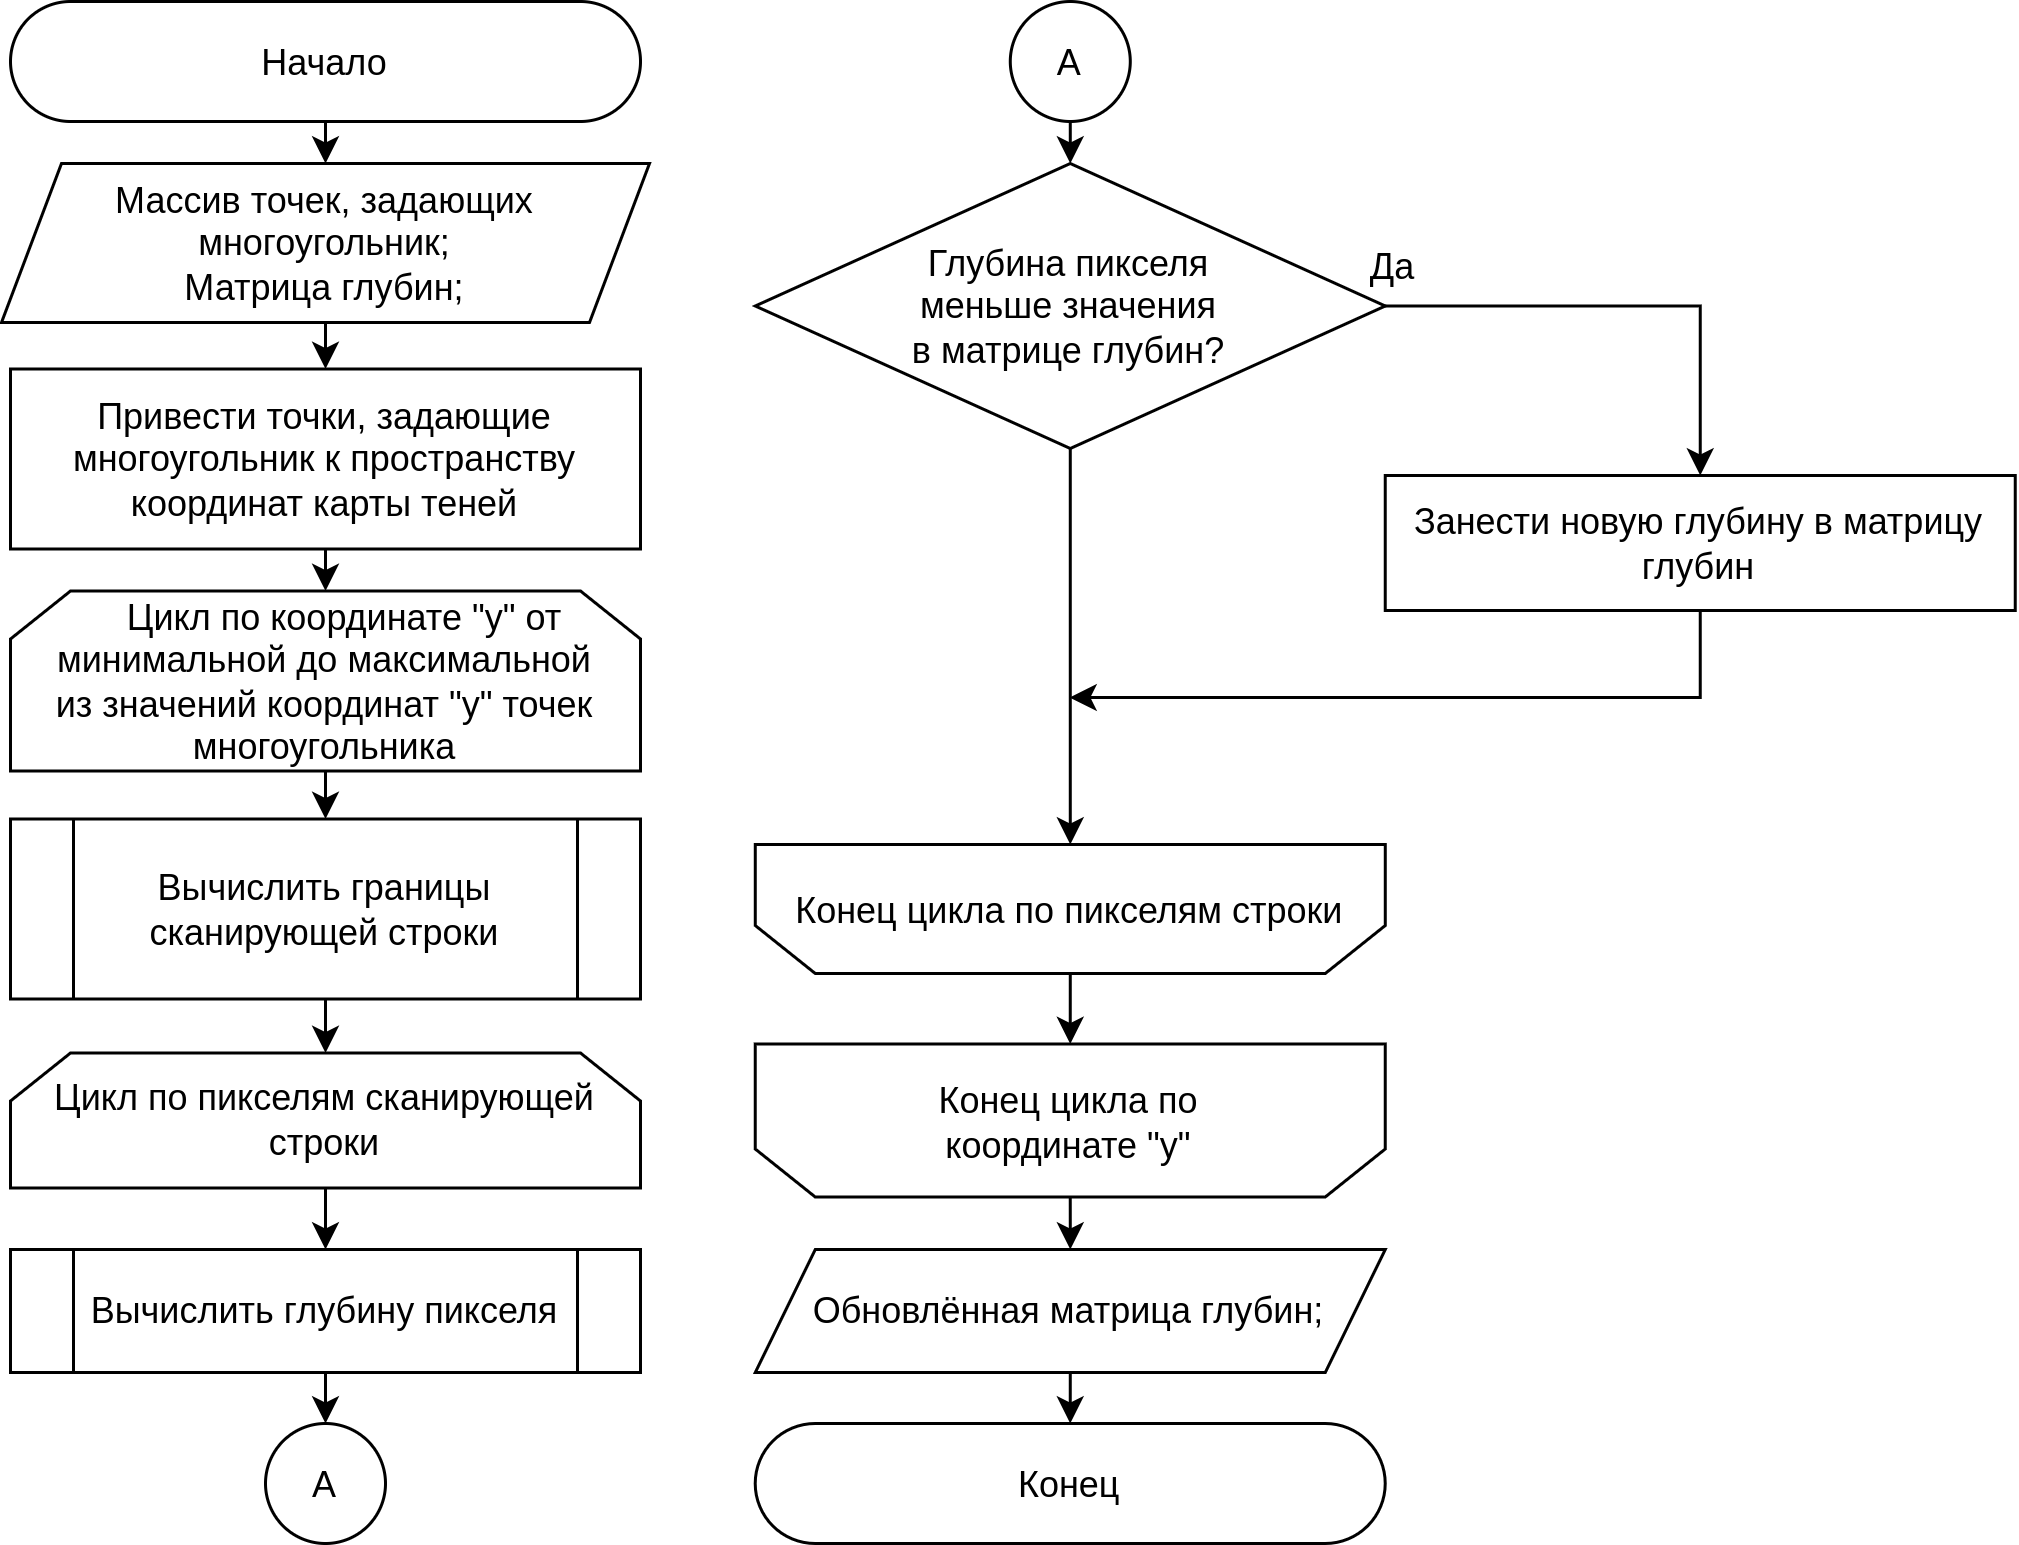
\includegraphics[height=.5\textheight]{smap.drawio.png}
  \caption{Алгоритм заполнения матрицы глубин для одного многоугольника}
  \label{fig:smap_buffer}
\end{figure}

Для вычисления цвета пикселя, находящегося в тени, используется формула~\eqref{eq:shadow}:

\begin{equation}
  \label{eq:shadow}
  \begin{split}
    r_1 = r*p \\
    g_1 = g*p \\ 
    b_1 = b*p
  \end{split}
  \end{equation}

, где $r_1, g_1, b_1$ --- значения интенсивности красного, зелёного и синего каналов цвета пикселя после затенения соответственно; $p$ --- коэффициент затенения; $r, g, b$ --- значения интенсивности красного, зелёного и синего каналов цвета исходного пикселя соответственно.

В данной работе был выбран коэффициент затенеия $p = 0.4$.


